\chapter{Software} \label{chap:software}
\begin{chapquote}{Norman Ralph Augustine, \textit{Augustine's Laws}}
Software is like entropy. It is difficult to grasp, weighs nothing, and obeys the Second Law of Thermodynamics; i.e., it always increases.
\end{chapquote}

As described in \Cref{sec:hw-control}, the hardware design of FPsPIN exposed all slow-path control flows to the host CPU through the \texttt{pspin\_\-ctrl\_\-regs}.  While this simplified the hardware design by allowing us to omit a dedicated \emph{management core} on the \ac{fpga}, the job of configuring the hardware now lands on the host CPU.  In addition, we also extended the handler runtime on PsPIN to support the new hardware integration.  We explain in this chapter the different software components developed for FPsPIN.  Three classes of software are required for the full operation of the hardware: Linux kernel modules, user-space library and utilities, and the updated handler runtime.  An overview of the software landscape of FPsPIN can be seen in \Cref{fig:sw-overview}.

\begin{figure}
    \centering
    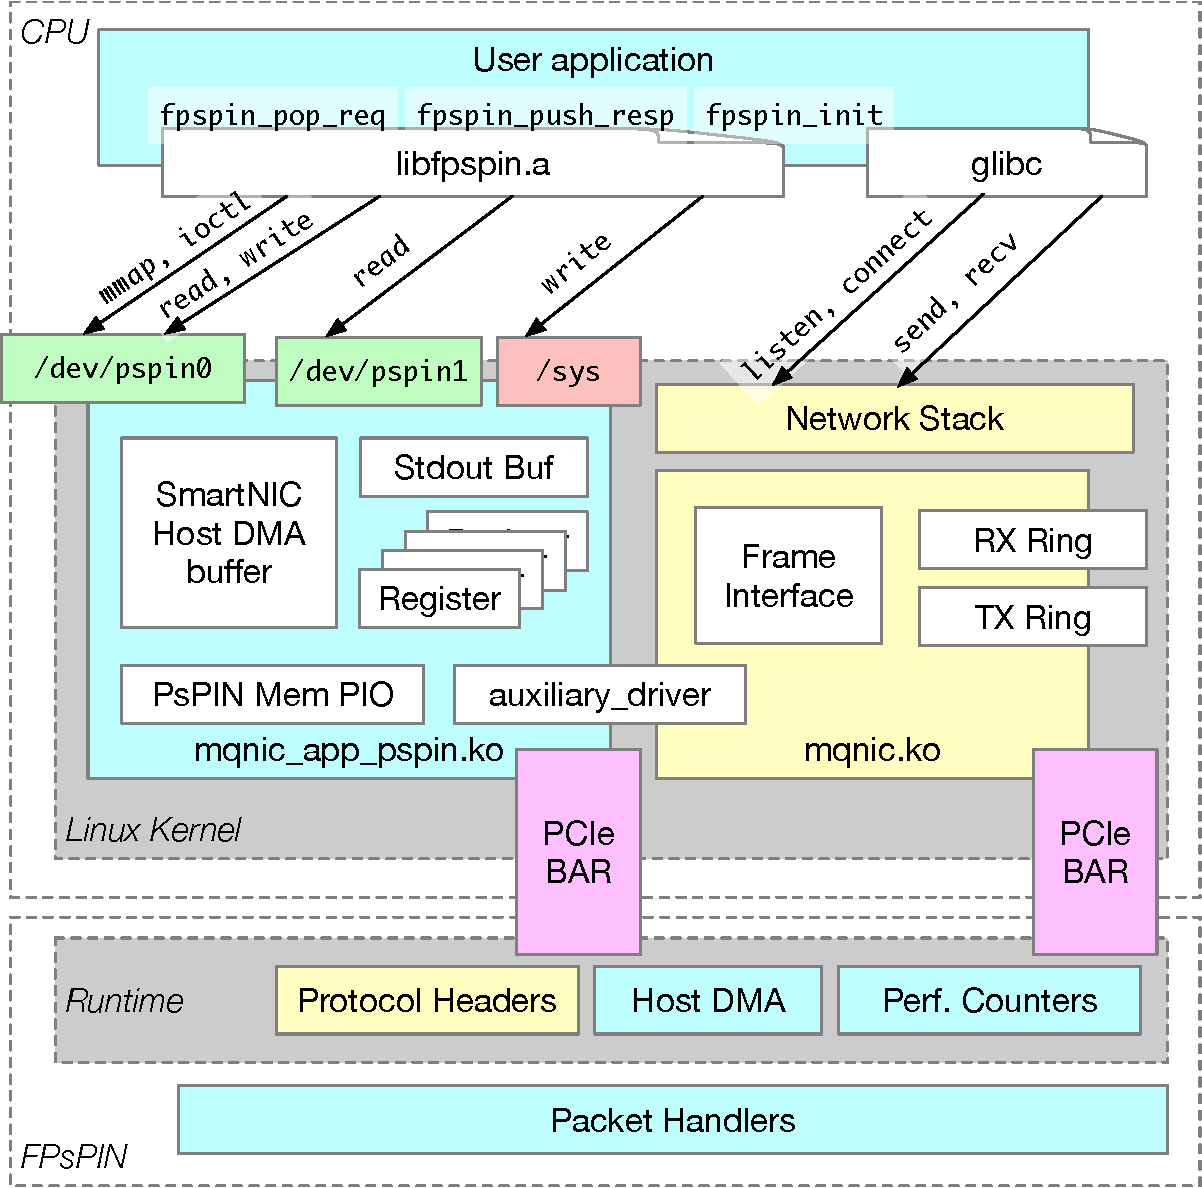
\includegraphics[width=.8\linewidth]{figures/sw-overview.pdf}
    \caption{Overview of the software on the host.  Yellow blocks denote existing software, while blue boxes show software developed in this project's scope.  Note that we use only standard Unix syscalls (\texttt{read}, \texttt{write}, \texttt{mmap}, \texttt{ioctl}) between the user- and kernel-space.} \label{fig:sw-overview}
\end{figure}

\section{CPU Kernel Modules} \label{sec:sw-kmod}

Linux is the major operating system used in diverse situations and is also used on the host by FPsPIN (in contrary, PsPIN runs bare-metal and does not have an operating system).  Multiple approaches to access to device memory exist and most of them require some degree of kernel-level support.  One approach is to expose device I/O memory access (in the case of \ac{pcie} devices, the \ac{bar}) to user-space through \texttt{/dev/mem} and host memory \ac{dma} access through \texttt{udmabuf}~\cite{ichiro_u-dma-bufuser_2023}.  While this approach is commonly used when developing \ac{fpga}-based accelerators in embedded environments, it introduces severe security risks due to exposing direct physical memory access to the user-space and is thus limited to embedded systems.

The other approach is to have a dedicated kernel module that interfaces with existing subsystems in Linux and does not expose unconstrained physical memory read and write (other than for diagnostics purposes).  The \ac{api} exposed by the device driver kernel module not only greatly reduces the attack surface, but also abstracts away details of the hardware between different revisions, facilitating development of user applications and support libraries.  While writing a dedicated kernel module requires experience with kernel programming, we argue that this is a necessity in hardware development for this thesis.  In addition, the overhead of doing so has already been greatly reduced by Corundum from their application block driver templates.  This is the approach adopted by Corundum (\texttt{mqnic.ko}) and in turn by FPsPIN (\texttt{mqnic\_\-app\_\-pspin.ko}) in this thesis.  

\subsection{mqnic.ko}

Corundum ships a kernel driver for the complete \ac{nic} functionalities, including interactions with the Linux network stack to expose the device as Ethernet \ac{nic}s for packet transmit and receive, as well as control interfaces with \texttt{ethtool} that reports link status.  In addition, it also exposes a device file \texttt{/dev/mqnicX} for the user-space libraries and utilities to perform management tasks, such as online firmware upgrade and device reset control.

Corundum provides driver support for the custom application block through the \emph{auxiliary bus} framework~\cite{noauthor_auxiliary_nodate} in Linux.  The framework allows splitting drivers for largely independent functionalities on the same device into different device drivers and thus different modules to allow compartmentalisation and separated operation.  The main device driver registers an auxiliary \emph{device} while the sub-component driver registers an auxiliary \emph{driver} with the framework.  In Corundum, the main driver registers the application block as an auxiliary device and exposes the \emph{application base address} (a separate \ac{pcie} \ac{bar}) to the auxiliary driver.  This allows the custom driver to access the application block \ac{bar} to interact with the hardware.

\subsection{mqnic\_\-app\_\-pspin.ko} \label{sec:app-kmod}

The driver for FPsPIN configures the PsPIN cluster and additional datapath components after they are brought out of reset.  The driver exposes two device nodes, \texttt{/dev/pspin\{0,1\}}, as well as a selection of device registers over \texttt{sysfs}~\cite{mochel_sysfs_2011}.  All user-space operations during configuration and normal operation happen through access to these resources using standard \emph{system calls} (syscalls).  In addition to normal operation, the kernel module checks for additional requirements imposed by the hardware and rejects requests from the user-space that violates these requirements.  We explain the main functionalities of the kernel module in this section.

\paragraph{Control registers} The control registers from the hardware are exposed as access to the \emph{application base address} from the Corundum auxiliary device.  We use the register generator introduced in \Cref{sec:hw-control}, \texttt{regs-compiler.sh}, to generate the respective sysfs node implementations; the register group and subgroup hierarchies are directly translated into \emph{device attributes}.  The generative approach keeps the driver's view of the device registers consistent with actual hardware.  We implement consistency checks of data-path engines via internal flags that are kept in sync with the respective enable registers, such that only valid and consistent configurations can be latched into hardware.

By exposing the hardware registers directly to user-space through sysfs, we adopt a \emph{user-space-centric} approach to hardware configuration.  This means that most configuration logic will be implemented in a user-space library (\Cref{sec:sw-lib}) instead of directly baked into the kernel module.  This allows more flexibility in the implementation, since we do not need to update the kernel module as often; it acts more as a \emph{shim} that only enforces basic safety and forwards other requests directly to the hardware.  This approach also offers more protection against programming errors when implementing the configuration routines, as errors in the user-space cannot crash the kernel.

\paragraph{Standard output read-back} Recall that as described in \Cref{sec:hw-control}, the \ac{hpu}s write their standard output into a \ac{fifo} for the host CPU to read for diagnostic purposes.  The FPsPIN kernel driver exposes the \texttt{/dev/pspin1} character device to the user-space.  For simplicity, the raw word sequence read from the hardware \ac{fifo} is directly exposed: each 4-byte word encodes one character as well as which \ac{hpu} wrote this character.  A user-space script later introduced in \Cref{sec:sw-lib} would de-multiplex this stream and write a log file for each \ac{hpu}.

In the current design and implementation, the standard output device file is \emph{on-demand}, meaning that data will be fetched from the \ac{fifo} only when a user-space program reads from the device file.  This has the potential issue of the \ac{hpu}s writing too fast to overflow the \ac{fifo}, resulting in a partially lost and corrupted output buffer.  An alternative design is to run a kernel \emph{worker} (also known as a kernel thread) that continuously polls on the hardware \ac{fifo} and actively fetches the standard output data as soon as it is available.  However, this would result in a constant overhead for busy polling and wouldn't be ideal if we do not care about the debug output.  We thus stick to the current on-demand design.

\paragraph{PsPIN memory access} As part of the configuration process, the host needs to download the code and runtime data for the \ac{hpu}s onto \ac{nic} memory.  As explained in \Cref{sec:hw-control}, a technicality due to the small Corundum control port address space mandates a static address mapping when accessing PsPIN memory from the host.  The kernel module implements this mapping and maintains the plain address view assumed by the PsPIN \ac{sdk}; requests that does not land in a valid memory area will be rejected with a SIGBUS (bus error signal in Linux) to avoid disrupting the hardware.  We hide the translation technicality away and never expose the exact mapping details to the user-space.

The kernel module exposes two \emph{flavours} of \ac{api}s to the user-space for accessing PsPIN memory, designed for different use cases.  The first flavour conforms to the traditional non-buffered Unix file I/O: we implement the \texttt{open()}, \texttt{seek()}, \texttt{read()}, \texttt{write()}, and \texttt{close()} syscalls on the \texttt{/dev/pspin0} character device.  Reads and writes to the device file are directly translated into reads and writes in the \ac{nic} memory region.  This flavour is suitable for bulk read or write on the PsPIN memory area and would be used during program image load or debug memory dumping.  It allows existing, unmodified Unix user-space utilities such as \texttt{dd}~\cite{noauthor_ieee_2018} to work as diagnosis tools and quick prototypes.

The second flavour is implemented as \texttt{ioctl()} over the \texttt{/dev/pspin0} device file.  An \emph{ioctl} (input/output control) is a syscall for device-specific I/O operations.  The syscall allows the user-space application to pass a pointer to the kernel to read or modify, along with an \emph{ioctl number} to denote the operation desired.   We implement two \emph{ioctls}, \texttt{PSPIN\_\-HOST\_\-WRITE} and \texttt{PSPIN\_\-HOST\_\-READ}, allowing the user-space to read and write 64-bit words in one action.  This simplifies the implementation of host \ac{dma} and performance counters user-space routines (\Cref{sec:sw-lib}) and reduces the syscall overhead.  In comparison, the traditional Unix file I/O approach would require two separate syscalls (\texttt{seek()} and \texttt{read()} or \texttt{write()}).

\paragraph{Host \ac{dma}} Memory pages used for \ac{dma} on Linux have to be registered with the kernel to ensure that cache coherency and alignment requirements are fulfilled.  It is also important to make sure that the memory page used for \ac{dma} are not moved by the kernel through swapping or memory compaction (through \texttt{kcompactd}).  The easiest way to ensure these requirements is to have the kernel module allocate the \ac{dma} buffer through the \ac{dma} \ac{api}, which takes care of these requirements automatically.  We implement the \texttt{mmap()} syscall for the \texttt{/dev/pspin0} device to perform a \emph{multi-use} \ac{dma} allocation (as opposed to \emph{single-use}; termed as \emph{coherent} by Linux, but does not actually imply cache coherency).  We then mark the area as \emph{uncached} and map the allocated \ac{dma} memory area into the user application address space to allow user processing of host \ac{dma} traffic.

Since we adopt a user-space-centric approach regarding the configuration registers, the user-space needs access to the physical address\footnote{On a system with an \emph{I/O memory management unit} (IOMMU) enabled, this is actually the \emph{bus} address as seen by the \ac{dma} bus masters in the device.} of the mapped \ac{dma} area to write to the control registers.  We implement another \emph{ioctl} on \texttt{/dev/pspin0}, \texttt{PSPIN\_\-HOST\ac{dma}\_\-QUERY}, to allow the user-space to query the physical address of the \ac{dma} area, in order to program the execution context to the data-path engines, specifically the \ac{her} generator.

The multi-use \ac{dma} buffer allocations we use suit the purpose of a \ac{dma} buffer shared between the CPU and device over a rather long period of time.  However, in the practice of implementing \ac{nic} drivers, the \emph{single-use} allocation scheme is more commonly used and allegedly more performant due to the possibility of taking advantage of the cache.  It is possible to take advantage of this approach in FPsPIN by using a separate \ac{dma} area per \emph{message}, as opposed to the current strategy of one area per \emph{execution context}.  We discuss a possible implementation in \Cref{sec:host-dma-qp} as future work.

\section{CPU User-Space} \label{sec:sw-lib}

The user-space software for FPsPIN caters to three distinct purposes in system operation: \emph{configuration} of the system to bring it into operative state; \emph{runtime} that supports the host-side application to interact with the \ac{nic}; and several \emph{utilities} to aid system-wide setup as well as to perform troubleshooting.  They interact with the various facilities provided by the \texttt{mqnic\_\-app\_\-pspin.ko} kernel module.  The user-space software shipped with FPsPIN are either packaged into a static library, \texttt{libfpspin.a}, along with the header files, or as standalone programs or scripts.

\paragraph{Configuration} The main configuration routine is packaged in \texttt{libfpspin.a} as one function: \texttt{fpspin\_init}.  It takes as input the device node exposed by the kernel (by default \texttt{/dev/pspin0}), the separately-built \ac{spin} handlers image, the ID of the execution context to use, and a number of rule sets for the matching engine.  The user can either select existing rule sets that match against common protocols, e.g.\ \ac{tcp} or \ac{udp} over IP/Ethernet, or define their own rule sets by filling in the \texttt{fpspin\_\-ruleset\_\-t} struct that contains configurations for each matching unit (review \Cref{sec:ingress-datapath} for more details).  \texttt{fpspin\_init} configures all the device registers over sysfs, loads the \ac{spin} handler image, and also allocates the host \ac{dma} area by requesting through \texttt{mmap} upon the kernel.  It then fills in all necessary addresses and handles in the context variable \texttt{fpspin\_\-ctx} and returns this to the user.  All future interactions with the runtime takes the context as an argument.

After a successful return of \texttt{fpspin\_\-init}, FPsPIN is ready for packet processing.  However, in complicated applications e.g.\ the datatypes demo shown in \Cref{sec:mpi-datatypes-demo},  the user may wish to perform additional initialisation, e.g., loading dynamically generated data into the \ac{nic} memory.  This is accomplished via the host access to \ac{nic} memory interfaces provided in \texttt{libfpspin.a}, namely \texttt{fpspin\_write\_memory}, allowing the host to generate the \ac{nic} memory content \emph{in} the host application at runtime.  The host application needs to take care of \emph{relocation} so that data structures contain valid \ac{nic} pointers when they are accessed by the \ac{hpu} in operation.

While the basic initialisation via \texttt{fpspin\_\-init} programs the matching engine as the last step such that no packets can arrive at the cluster until it is fully configured, host-side user initialisation happens after the \ac{hpu}s have started execution.  As a result, the user needs to ensure that the \ac{spin} handlers do not start processing packets until the host initialisation process is finished, e.g.\ through a flag that gates all \ac{hpu}s from running.  The exact mechanism and interface requirements are further discussed in \Cref{sec:handler-init} as a possible extension to the \ac{spin} specification.

\paragraph{Runtime} If the \ac{spin} packet handlers programmed to the cluster requires interaction with the host, e.g.\ to forward a processed incoming message to the host for further processing, the host application should then \emph{poll} the notification interface from time to time.  We currently implement a simple flag-based notification method as shown in \Cref{fig:host-dma-req-resp}: both PsPIN and the CPU writes \emph{remotely} and polls \emph{locally}.  The host application tries to pop a notification from PsPIN using \texttt{fpspin\_\-pop\_\-req} (\circled{2}).  If a message is present, the host application processes the message and sends back a response via \texttt{fpspin\_\-push\_\-resp} (\circled{3}).  The rest of the process (\circled{1}, \circled{4}) happens in the handler runtime to be introduced in \Cref{sec:handler-runtime}.

It is important that the host CPU should be able to perform other workloads, such as computational tasks, during packet processing in a truly \emph{offloading} manner.  The host application can overlap other workloads via multi-threading or by anticipating the \ac{img} and polling only when there could be a message arriving.  For simplicity, the current flags-based host \ac{dma} notification facility can only hold one in-flight message between the host and each \ac{hpu}; this limits the duration of overlapped workloads between polling to be one \ac{img}.  The overlap can be increased by implementing a proper ring buffer for the notification, which we leave as a possible future improvement.

\begin{figure}[tp]
    \centering
    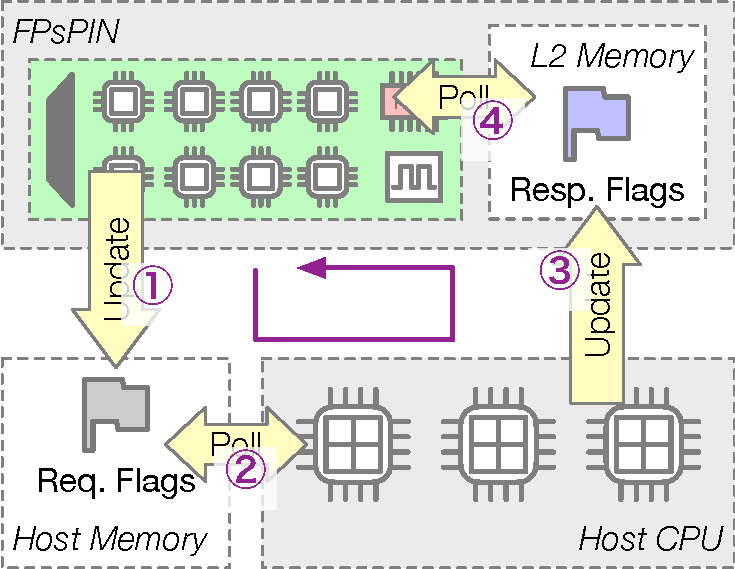
\includegraphics[width=.5\textwidth]{thesis/figures/host-dma-req-resp.pdf}
    \caption[Simplified view of the host \ac{dma} loop]{Simplified view of the host \ac{dma} loop, in chronological order.  \circled{1}) The \ac{hpu} sends a request to the host for processing, by writing to the flag in host memory; \circled{2}) the host polls and pops the request from local memory; \circled{3}) the host pushes the response by writing to the flag in \ac{nic} memory; \circled{4}) the \ac{hpu} polls and pops the response from local memory.} \label{fig:host-dma-req-resp}
\end{figure}

The host application may still need to receive and send network packets on the same interface, for example to implement the slow, non-performance-critical paths of a network protocol, like connection setup and tear-down in \ac{tcp}.  The intended operation for this purpose is via the host network stack, either normally or through the \emph{raw} sockets (in case of state confusion due to partially offloaded messages).  The user needs to correctly configure the matching engine, so that these packets are actually delivered to the host CPU and not to PsPIN.  Alternatively, if it is difficult to express the criteria in the matching rules, the user can make the handlers perform a \emph{secondary match} and deliver such packets to the host over host \ac{dma}.

Performance measurements are important to estimate bottlenecks of packet processing.  The runtime provides facility to read and clear \emph{performance counters} exposed by the handlers.  Up to 16 32-bit counters are accessible from the host application via \texttt{fpspin\_\-get\_\-counter} and \texttt{fpspin\_\-clear\_\-counter}.  Each counter keep track of a total sum and iteration count of updates, enabling the calculation of an average value.  The counters are updated in the packet handlers using a facility in the handler runtime.

\paragraph{Utilities} In addition to the \texttt{libfpspin.a} library to be statically linked into the user application, we also provide several standalone utilities that are important to the normal operation of FPsPIN.  One of these is \texttt{cat\_stdout.py} that reads from the log facility, \texttt{/dev/pspin1}, provided by the application kernel module.  The script performs \emph{blocking read} on the log device and demultiplexes the stream of printed characters according to the core ID.  The user can specify whether to dump the log to files and if the script should remove stale logs.  The script is provided separately instead of integrated into the runtime, in case of an application that does not care about the debug output from the \ac{hpu}s and thus does not want to waste CPU cycles to read them.

During the development and testing of handlers, it may be necessary to read or write specific memory locations in the \ac{nic} L2 memory.  The \texttt{mem} utility takes a \ac{nic} address and performs a 64-bit read or write command over the \texttt{ioctl} interface provided by the kernel module.  It is possible to implement a more complicated debugger protocol with memory access in this fashion; we leave this as future work.

\section{Handler Runtime} \label{sec:handler-runtime}

The PsPIN project provided a rather comprehensive implementation of the handler-side \ac{spin} \ac{api} through the PsPIN/PULP runtime.  This includes the \ac{her} and task data structures, as well as host \ac{dma} commands for the handler code to invoke.  A few additions are made to accomodate new abstractions introduced by FPsPIN.  One of such additions concerns packet header processing.  The existing PsPIN runtime already provides C structs for interpreting headers for IP and \ac{udp}, but since FPsPIN directly receives Ethernet frames instead of the IP payloads of a lower-level messaging network layer e.g.\ \ac{ipoib}, we added the Ethernet header and \ac{mac} address structs for this situation.  We also implement support for the \ac{slmp}, introduced later in \Cref{sec:slmp}, in the same manner in the FPsPIN runtime.

As we have seen in \Cref{fig:host-dma-req-resp}, the handler issues notifications to the host for \ac{dma} events and pops the response of the host.  The handler, through the runtime function \texttt{fpspin\_\-host\_\-req}, issues the host notification via a host \ac{dma} write (\circled{1}) and polls for the host response in local memory (\circled{4}).  The location of the host flag sits at a pre-determined offset in the host \ac{dma} area, while the \ac{nic} flag is exposed via a global symbol in the handler image, retrieved during loading.  Note that we adopt a \emph{synchronous} design here in contrast to the \emph{asynchronous} design for the host-side counterpart of the host \ac{dma} process.  This is currently justified since most of the host notifications happen at the end of messages in the \emph{tail} handler and the handler would not have meaningful workload to overlap with.

\paragraph{Performance measurements} The host-side runtime has support for reading back performance counters generated by the handler routines; these counters are updated through the handler runtime on the \ac{hpu}.  Each 64-bit counter consists of two 32-bit fields, the \emph{sum} and \emph{count}, allowing the handler logic to push a specific performance value into the counter with the \texttt{push\_\-counter} routine.  Every time the counter is incremented, the count field is incremented by one.  The counters sit in L2 memory accessible to the host and are initialised to zero on cluster setup.  These counters can be used to collect various statistics such as handler execution time at handler or message granularity,  as well as to profile specific code areas in the handler routines. 

The counter values for performance measurements are derived from the \emph{cycles} register in \ac{pulp} that is only accessible to \emph{machine-mode}, while the handler code executes in user-mode.  We extend the existing fault handler in the PsPIN runtime to handle syscalls and implement a syscall to read the cycles register.  With the current na\"ive implementation, this syscall path takes around 100 cycles on the \ac{pulp} cores, in which most of the time consumed comes from the need to save and restore all general purpose registers.  While it is possible to optimise this path for a lower latency, a proper solution is to address the lack of a user-accessible time register for precise performance measurements as we will argue in \Cref{sec:telemetry-introspection}.  We leave the related changes to hardware as future work.